\newpage
\section{Interference}

Optics and Gravitation: Massive galaxies/black holes act like special lenses. 

\subsection{The Superposition of Waves}
The pheenomena of interference , diffraction and polarization share a commom conceptual basis in that they deal with two or more light waves overlap in some region of space. 

Recall that each field component of an electromagnetic wave $(E_{xyz}, B_{xyz})$ satisfies the scalar 3D differential wave equation
\begin{align*}
    \frac{1}{v^2}\frac{\partial^2 \psi }{\partial t^2}=&\frac{\partial^2 \psi }{\partial x^2}+\frac{\partial^2 \psi }{\partial y^2}+\frac{\partial^2 \psi }{\partial z^2}\\
    =&\nabla^2\psi
\end{align*}

This equation is \highlight{linear}, $\psi(\vec{r},t)$ and its derivatives appear only to the first power. Consequently, if $\psi_i(\vec{r},t)$ are solutions, any \highlight{linear combination} of them 
\begin{align*}
    \psi(\vec{r},t)=\sum_{i=1}^n C_i \psi_i(\vec{r},t)
\end{align*}
will be a solution as well. 

\subsubsection{Examples od Superposition}
\begin{enumerate}
    \item Beats: Two harmonic waves of different frequency traveling in the same direction.
    \begin{align*}
        \psi=\psi_1+\psi_2=A\cos\omega_1 t + A\cos \omega_2 t, \, \omega_1\approx \omega_2 
    \end{align*}
    \item Standing waves: Two harmonic waves of the same frequency propagating in opposite directions.
    \begin{align*}
        \psi=\psi_1+\psi_2=A\cos(kx-\omega t)-A\cos(-kx-\omega t)
    \end{align*}
\end{enumerate}

\subsubsection{The Algbraic Method of Adding Waves}
There are several equivalent ways of mathematically adding two or more overlapping waves that have \highlight{the same frequency and wavelength}. 

Suppose there are two such waves 
\begin{align*}
    E_1=E_{01}\cos\left( \alpha_1-\omega t \right)\\
    E_2=E_{02}\cos\left( \alpha_2-\omega t \right)
\end{align*}
where 
\begin{align*}
    \alpha_i=kx_i+\phi_i
\end{align*}
with $x_i$ being the distance from the source $s_i$ of the wave to the point of observation. 

The linear combination of the waves is 
\begin{align*}
    E\equiv E_0\cos\left( \alpha-\omega t \right) = E_1+E_2
\end{align*}
where (notice $\cos\omega t$ and $\sin\omega t$ are linearly independent)
\begin{align*}
    E_0\cos \alpha &=E_{01}\cos\alpha_1+E_{02}\cos\alpha_2\\
    E_0\sin \alpha &=E_{01}\sin\alpha_1+E_{02}\sin\alpha_2
\end{align*}
and
\begin{align*}
    E_0^2=E_{01}^2+E_{02}^2+2E_{01}E_{02}\cos\left( \alpha_2-\alpha_1 \right)
\end{align*}

$2E_{01}E_{02}\cos\left( \alpha_2-\alpha_1 \right)$ is known as the \highlight{interference term (干涉项)}.

The crucial factor is the \highlight{phase difference (相位差)} bewteen the two interfering waves $E_1$ and $E_2$, 
\begin{align*}
    \delta \equiv \left( \alpha_2-\alpha_1 \right)=\frac{2\pi}{\lambda}(x_2-x_1)+(\phi_2-\phi_1)
\end{align*}

\begin{itemize}
    \item When $\left( \alpha_2-\alpha_1 \right)=2m\pi$ for integer $m$, we have 
    \begin{align*}
        E_0^2=E_{01}^2+E_{02}^2+2E_{01}E_{02}
    \end{align*}

    In particular, $E_0=4E_{01}^2$ when $E_{01}=E_{02}$. The two waves interfere constructively. 
    \item When $\left( \alpha_2-\alpha_1 \right)=(2m+1)\pi$ for integer $m$, we have
    \begin{align*}
        E_0^2=E_{01}^2+E_{02}^2-2E_{01}E_{02}
    \end{align*}

    In particular, $E_0=0$ when $E_{01}=E_{02}$. The two waves interfere destructively. 
\end{itemize}

\subsubsection{The Complex Method}
Above all, 
\begin{align*}
    e^{i\theta}=&\cos\theta+i\sin\theta\\
    (e^{i\theta})^*=&e^{-i\theta}
\end{align*}

The wave function
\begin{align*}
    E_1=&E_{01}\cos\left( \alpha_1-\omega t \right)\\
    =&E_{01}\cos\left( kx_1-\omega t +\phi_1\right)
\end{align*}
can be written as 
\begin{align*}
    \tilde{E}_1=&E_{01}e^{i(\alpha_1-\omega_1 t)}\\
    =&E_{01}e^{i\alpha_1}e^{-i\omega_1 t}
\end{align*}
if we are interseted only in the real part. 

Suppose that there are two such overlapping waves having the same frequency and traveling in the positive x-direction. The resultant wave is given by
\begin{align*}
    \tilde{E}=\highlight{E_{0}e^{i\alpha}}e^{-i\omega t}=\left[ \highlight{E_{01}e^{i\alpha_1}+E_{02}e^{i\alpha_2}} \right]e^{-i\omega t}
\end{align*}
where $E_{0}e^{i\alpha}$ is known as the complex amplitude of the composite wave. 

Since $E_0^2=\left( E_0e^{i\alpha} \right)^*\left(E_0e^{i\alpha}\right)$,  we find
\begin{align*}
    E_0^2=&\left[ E_{01}e^{-i\alpha_1}+E_{02}e^{-i\alpha_2} \right]\left[ E_{01}e^{i\alpha_1}+E_{02}e^{i\alpha_2} \right]\\
    =&E_{01}^2+E_{02}^2+E_{01}E_{02}\left[ e^{i(\alpha_2-\alpha_1)} + e^{-i(\alpha_2-\alpha_1)} \right]\\
    =&E_{01}^2+E_{02}^2+2E_{01}E_{02}\cos(\alpha_2-\alpha_1)
\end{align*}

\subsubsection{Phasor Addition}

\begin{figure}[H]
    \centering
    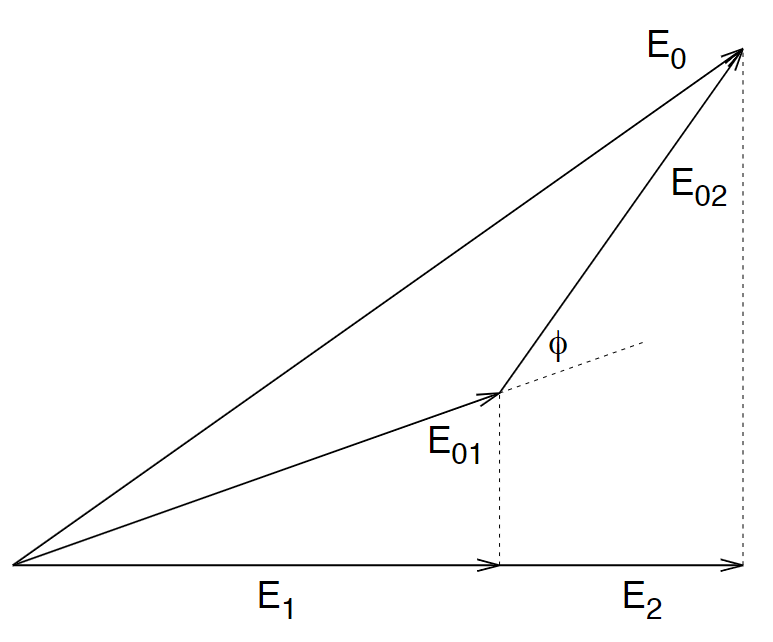
\includegraphics[width=0.42\textwidth]{Lec17/Phasor Addition}
    \caption{Phasor Addition}
\end{figure}

We represent a wave, which has an amplitude and a phase, to a vector, know as a \highlight{phasor}, in a two-dimensional plane, such that
\begin{align*}
    E_i=&E_{0i}\cos(\alpha_i-\omega t)\\
    =&\left(E_{0i}\cos\alpha_i\right)\cos\omega t+\left(E_{0i}\sin\alpha_i\right)\sin\omega t\\
    \Longrightarrow\vec{E}_i=&\left(E_{0i}\cos\alpha_i\right)\hat{x}+\left(E_{0i}\sin\alpha_i\right)\hat{y}
\end{align*}

The algebraic sum, $E=E_1+E_2$ is the projection on the x axis of the corresponding phasor sum. 

If we denote the phase delay $\phi=\alpha_2-\alpha_1$ as shown in the \highlight{phasor diagram}, the law of cosines applied to the triangle of sides $\vec{E}_{01}$, $\vec{E}_{02}$ and $\vec{E}_{0}$ yields 
\begin{align*}
    E_0^2=E_{01}^2+E_{02}^2+E_{01}E_{02}\cos(\alpha_2-\alpha_1)
\end{align*}


\subsection{Young's Double-Slit Interference Experiment}

\subsubsection{Natural Light}
The light from two fine incandescent wires wouldn't interfere, because the light is emitted by vast numbers of atoms in the wires, acting randomly and independently for extremely short times --- of the order of nanoseconds. The light is said to be \highlight{incoherent (不相干, 离散)}. As a result, at any given point on the viewing screen, the interference between the waves from the two sources varies rapidly and randomly between fully constructive and fully destructive. The screen is seen as being uniformly illuminated (over the time scale of our observation). 

Conditions for Interference: 
\begin{enumerate}
    \item Two beams must have (nearly) the same frequency $\omega$. therwise, the phase difference is time-dependent. During the detection interval, the interference pattern will be averaged away.
    \item The clearest pattern (with maximum contrast) exists when interfering waves have (nearly) equal amplitude. 
    \item Initial phase difference can exist between sources, as long as it remains constant; the two sources are said to be \highlight{coherent (相干, 一致)}.
\end{enumerate}

\subsubsection{Huygen's Principle}
lf waves strike a barrier with a small opening, the waves may be seen to expand from the opening Notice the wavelength is larger than the opening in this case. 

\begin{figure}[H]
    \centering
    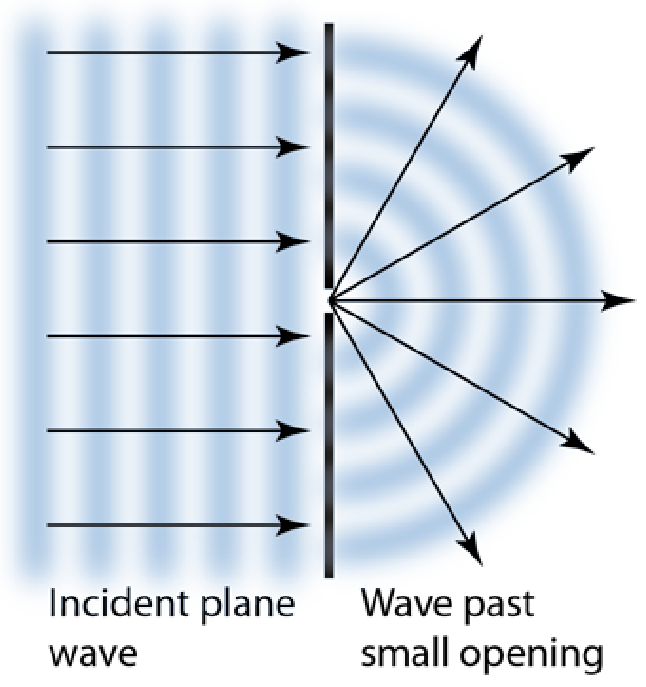
\includegraphics[width=0.28\textwidth]{Lec17/Huygen's Principle}
    \caption{Huygen's Principle}
\end{figure}

\subsubsection{Young's Interference Experiment}
Here is the ingenious arrangement of Thomas Young's double-slit experiment. 

\begin{figure}[H]
    \centering
    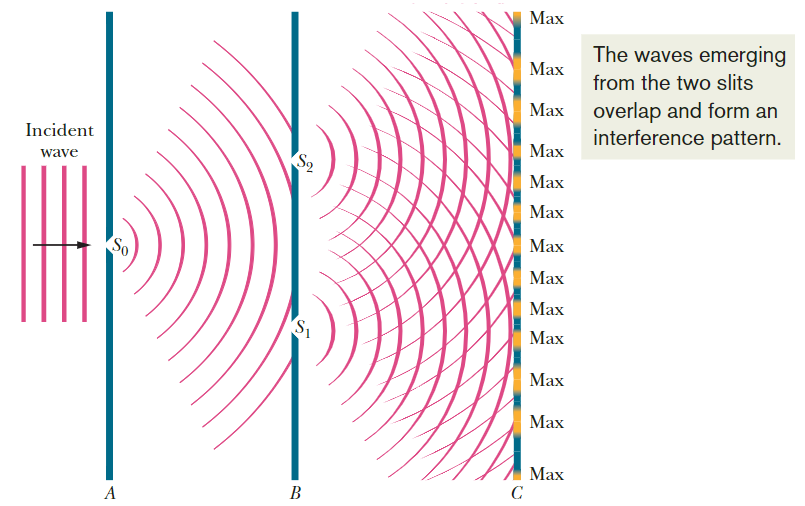
\includegraphics[width=0.47\textwidth]{Lec17/Young's Interference Experiment}
    \caption{Young's Interference Experiment}
\end{figure}

The slit $S_0$ in screen $A$ creats a spatially coherent beam that could identically illuminate slits $S_1$  and $S_2$ in screen $B$. Nowdays, plane waves from a laser can provide the spatial coherence the experiment needs. Finally, light waves produce fringes in a Young’s double-slit interference experiment. 

The waves are in phase (相同) when they pass through the two slits because there they are just portions of the same incident wave. However, once they have passed the slits, the two waves must travel different distances to reach point $P$ on screen $C$. The path length difference is, when $d\ll D$,
\begin{align*}
    \Delta L=d\sin\theta
\end{align*}

However, the electric field components of these waves at point $P$ are not in phase and vary with time as
\begin{align*}
    E_1=E_0\cos(kr_1-\omega t)=E_0\cos(kL+\beta -\omega t)\\
    E_2=E_0\cos(kr_2-\omega t)=E_0\cos(kL-\beta -\omega t)
\end{align*}
where the phase difference$\left[ L=\frac{r_1+r_2}{2}=\sqrt{D^2+y^2} \right]$
\begin{align*}
    \delta_2=2\beta=k\Delta L=\frac{2\pi d}{\lambda}\sin\theta
\end{align*}

The total intensity is thus given by 
\begin{align*}
    I=2E_0^2\left[ 1+\cos(2\beta) \right]=I_{max}\cos^2\beta
\end{align*}


\begin{figure}[H]
    \centering
    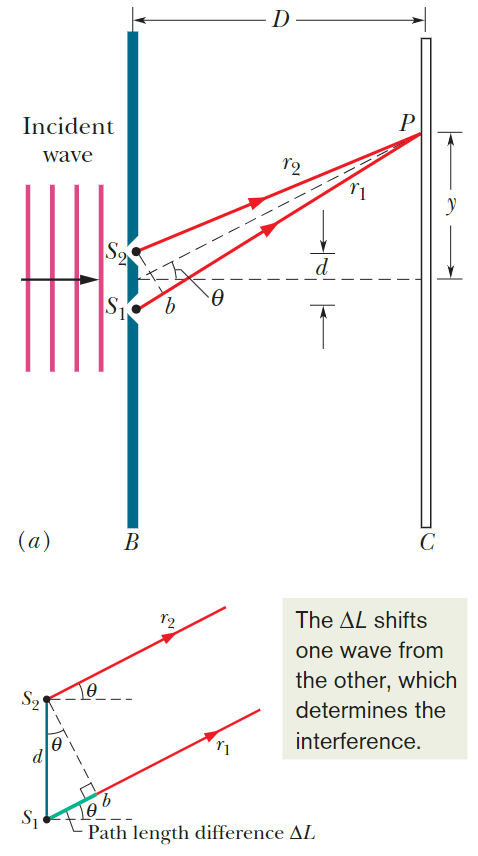
\includegraphics[width=0.209\textwidth]{Lec17/interference}
    \caption{The waves pass through the two slits}
\end{figure}

Therefore, a bright fringe appears when
\begin{align*}
    \Delta L=d\sin\theta=m\lambda
\end{align*}
when $m$ is an integer.

On the other hand, a dark fringe appears when 
\begin{align*}
    \Delta L=d\sin\theta = \left(m+\frac{1}{2}\right)\lambda
\end{align*}
where $m$ is an integer. 

We can then find the angle $\theta$ to any fringe and thus use the values of $m$ to label the fringes.

\subsection{Interference from Thin Films}
Consider a thin transparent film of uniform thickness $L$ and index of refraction $n_2$, illuminated by bright light of wavelength $\lambda$ from a distant point source. We assume $n_1=n_3=n_{air}$. For simplicity, we also assume that the light rays are almost perpendicular to the film $(\theta\approx 0)$. 

\begin{figure}[H]
    \centering
    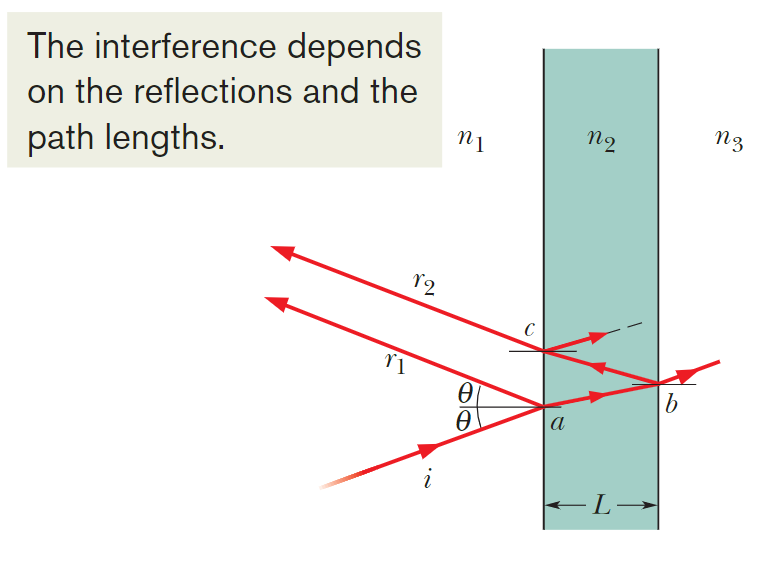
\includegraphics[width=0.309\textwidth]{Lec17/Interference from Thin Films}
    \caption{Interference from Thin Films}
\end{figure}

Reflection at an interface can cause a phase change (相变), depending on the indexes of refraction on the two sides of the interface. There is no phase change for refraction. The results for light reflecting off a medium can be summarized as 
\begin{table}[H]
    \centering
    \begin{tabular}[c]{|c|c|}\hline
        Reflection & Reflection phase shift\\ \hline
        Off lower index & 0\\
        Off higher index & 0.5 wavelength\\ \hline
    \end{tabular}
    \caption{light reflecting off a medium }
\end{table}

So reflecting off higher index, ray $r_1$ has an additional reflection phase shift 0.5 wavelength. There is no such shift for $r_2$. In addition, the light waves of rays $r_1$ and $r_2$ has a path difference $2L$, which occurs in index $n_2$. Notice the wavelength in the medium $(r_2)$ is 
\begin{align*}
    \lambda_2 =\frac{v_2}{f}=\frac{c}{n_2 f}=\frac{\lambda}{n_2}
\end{align*}
the $r_1$ and $r_2$ are $(k_2=\frac{2\pi}{\lambda_2})$
\begin{align*}
    \vec{E}_1=&E_0\cos\left(k\left(x+\frac{1}{2}\lambda\right)-\omega t\right)\\
    =&E_0\cos(\pi+kx-\omega t)\\
    \vec{E}_2=&E_0\cos(k_2 2L+kx-wt)\\
    \therefore \, \vec{E}^2 =&\left( \vec{E}_1+\vec{E}_2 \right)^2=2E_0^2\left(1+\cos(k_2 2L-\pi) \right)
\end{align*}

Therefore, rays are in phase if 
\begin{align*}
    (k_2 2L-\pi)&=2m\pi\\
    2L=\left(m+\frac{1}{2}\right)\lambda_2&=\left(m+\frac{1}{2}\right)\frac{\lambda}{n_2}
\end{align*}
for integer $m$. They produce an interference maximum and the nearby region on the film is bright to observers. 

Similarly, if they are exactly out of phase (不同相位)
\begin{align*}
    (k_2 2L-\pi)&=(2m+1)\pi\\
    2L=m\lambda_2&=m\frac{\lambda}{n_2}
\end{align*}
for integer $m$. They produce an interference minimum and the nearby region is dark, even though it is illuminated. 

\subsubsection{Negligible Film Thickness}
A special situation arises when a film is so thin that $L$ is much less than $\lambda$, say $L<0.1\lambda$. Then the path length difference $2L$ can be neglected, and the phase difference between $r_1$ and $r_2$ is due only to reflection phase shifts. Thus $r_1$ and $r_2$ are exactly out of phase, and thus the film is dark, regardless of the wavelength and intensity of the light. 